%============================ MAIN DOCUMENT ================================
% define document class
\PassOptionsToPackage{table}{xcolor}
\documentclass[
  a4paper,
  BCOR=15mm,            % Binding correction
  twoside,
% openright,
%  headings=openright,
  bibliography=totoc,   % If enabled add bibliography to TOC
  listof=totoc,         % If enabled add lists to TOC
  monolingual,
% bilingual,
  invert-title,
]{bfhthesis}

\LoadBFHModule{listings,terminal,boxes}
%---------------------------------------------------------------------------
% Documents paths
%---------------------------------------------------------------------------
\makeatletter
\def\input@path{{content/}}
%or: \def\input@path{{/path/to/folder/}{/path/to/other/folder/}}
\makeatother
%-----------------  Base packages     --------------------------------------
% Include Packages
\usepackage[french,ngerman,main=english]{babel}  % https://www.namsu.de/Extra/pakete/Babel.html

\usepackage{amsmath}          % various features to facilitate writing math formulas
\usepackage{amsthm}           % enhanced version of latex's newtheorem
\usepackage{amsfonts}         % set of miscellaneous TeX fonts that augment the standard CM
\usepackage{amssymb}          % mathematical special characters

\usepackage{siunitx}

\usepackage{graphicx}         % integration of images
\usepackage{float}            % floating objects

\usepackage{caption}          % for captions of figures and tables
\usepackage{subcaption}       % for subcaptions in subfigures
\usepackage{cite}             % use bibtex
\usepackage{wrapfig}

\usepackage{exscale}          % mathematical size corresponds to textsize
\usepackage{multirow}         % multirow emables combining rows in tables
\usepackage{multicol}

\usepackage{longtable}

\usepackage{parskip}



%---------------------------------------------------------------------------
% Graphics paths
%---------------------------------------------------------------------------
\graphicspath{{pictures/}{figures/}}
%---------------------------------------------------------------------------
% Blind text -> for dummy text
%---------------------------------------------------------------------------
\usepackage{blindtext}    
\usepackage{letltxmacro}   
\LetLtxMacro{\blindtextblindtext}{\blindtext}

\RenewDocumentCommand{\blindtext}{O{\value{blindtext}}}{
	\begingroup\color{BFH-Gray}\blindtextblindtext[#1]\endgroup
}
%---------------------------------------------------------------------------
% Glossary Package
%---------------------------------------------------------------------------
% the glossaries package uses makeindex
% if you use TeXnicCenter do the following steps:
%  - Goto "Ausgabeprofile definieren" (ctrl + F7)
%  - Select the profile "LaTeX => PDF"
%  - Add in register "Nachbearbeitung" a new "Postprozessoren" point named Glossar
%  - Select makeindex.exe in the field "Anwendung" ( ..\MiKTeX x.x\miktex\bin\makeindex.exe )
%  - Add this [ -s "%tm.ist" -t "%tmx.glg" -o "%tm.gls" "%tm.glo" ] in the field "Argumente"
%
% for futher informations go to http://ewus.de/tipp-1029.html
%---------------------------------------------------------------------------
\usepackage[nonumberlist]{glossaries-extra}
\makeglossaries
\newglossaryentry{BibTeX}{
  name={BibTeX},
  description={Program for the creation of bibliographical references and directories in \TeX or \LaTeX\, documents},
  plural=BibTeXs
}

\newglossaryentry{zynq}{
  name=Zynq,
  description={\textbf{Zynq} Xilinx' AP SoC. The characteristic feature of Zynq is that it combines a dual-core ARM Cortex-A9 processor with traditional Series-7 FPGA logic fabric},
  plural=Zynqs
}


\newglossaryentry{soc}{
  name=SoC,
  description={\textbf{System-on-Chip (SoC)} A single chip that holds all of the necessary hardware and electronic circuitry for a complete system. SoC includes on-chip memory (RAM and ROM), the microprocessor, peripheral interfaces, I/O logic control, data converters, and other components that comprise a complete computer system},
  plural=SoCs
}

\newglossaryentry{apsoc}{
  name=AP SoC,
  description={\textbf{All Programmable System-on-Chip (AP SoC)} was introduced by Xilinx. It represents a IC which comprise a hard-core processor core surrounded by an FPGA fabric. This type of ICs are highly configurable and provide algorithm partitioning capabilities. This provides high benefit for highly scale-able applications as well as fast time-to-market},
  plural=AP SoCs
}

\newglossaryentry{zbook}{
  name=Zynq Book,
  description={\textbf{Zynq Book} A book that summarizes all the important aspects when working with Zynq and provides a strong and easy understandable introduction to the topic. The book has been written by a team of University of Strathclyde Glasgow in cooperation with Xilinx},
  plural=Zynq Books
}

\newglossaryentry{zboard}{
  name=ZedBoard,
  description={\textbf{ZedBoard} A low cost development board featuring a Zynq-700 0 SoC, and a number of peripherals},
  plural=ZedBoards
}


\newglossaryentry{asic}{
  name=ASIC,
  description={\textbf{Application-Specific Integrated Circuit (ASIC)} An integrated circuit which is designed for a specific use, rather than general-purpose use},
  plural=ASICs
}

\newglossaryentry{rtos}{
  name=RTOS,
  description={\textbf{Real-Time Operating System (RTOS)} A category of operating systems defined by their ability to respond quickly and predictably for a given task},
  plural=RTOSs
}

\newglossaryentry{arm}{
  name=ARM,
  description={\textbf{ARM} A family of processor architectures. The hard processor type which forms the basis of the Zynq processing system is an ARM Cortex-A9 version. The term ‘ARM’ may also be used to refer to the developer of the processor, i.e. a company of the same name}
}

%---------------------------------------------------------------------------
% Makeindex Package
%---------------------------------------------------------------------------
\usepackage{makeidx}
\makeindex
%\usepackage{imakeidx}          % To produce index
%\makeindex[columns=2,intoc]    % Index-Initialisation
%\makeindex[columns=3,columnseprule,columnsep,intoc]
%---------------------------------------------------------------------------
% Hyperref Package (Create links in a pdf)
%---------------------------------------------------------------------------
\usepackage[
	,bookmarks
	,plainpages=false
	,pdfpagelabels
        ,pdfusetitle
	,backref = {false}          % No index backreference
	,colorlinks = {true}        % Color links in a PDF
	,hypertexnames = {true}     % no failures "same page(i)"
	,bookmarksopen = {true}     % opens the bar on the left side
	,bookmarksopenlevel = {0}   % depth of opened bookmarks
	,linkcolor=.
	,filecolor=.
	,urlcolor=.
	,citecolor=.
]{hyperref}
%---------------------------------------------------------------------------

%% %% Customize Footer and Headers in Document
%% \KOMAoptions{headsepline,plainheadsepline,footsepline,plainfootsepline}%
%% \setkomafont{headsepline}{\color{BFH-DarkBlue}}% BFH-DarkBlue required bfhcolors
%% \setkomafont{footsepline}{\color{BFH-DarkBlue}}%
%% \lehead*{lehead} % the * character does replace the header on the first chapter page as well
%% \cehead*{cehead}
%% \rehead*{rehead}
%% \lohead*{lohead}
%% \cohead*{cohead}
%% \rohead*{rohead}

%% \lefoot*{lefoot}
%% \cefoot*{cefoot}
%% \refoot*{refoot}
%% \lofoot*{lofoot}
%% \cofoot*{cofoot}
%% \rofoot*{rofoot}
%---------------------------------------------------------------------------
\begin{document}

%------------ START FRONT PART ------------
\frontmatter

\title{Projekt 2}
\subtitle{AR / POSE Estimation}
\author{Bernhard Messerli}
\institution{Bern University of Applied Sciences}
\department{Technik und Informatik}
\institute{Informatik}
\version{1.0}
\titlegraphic*{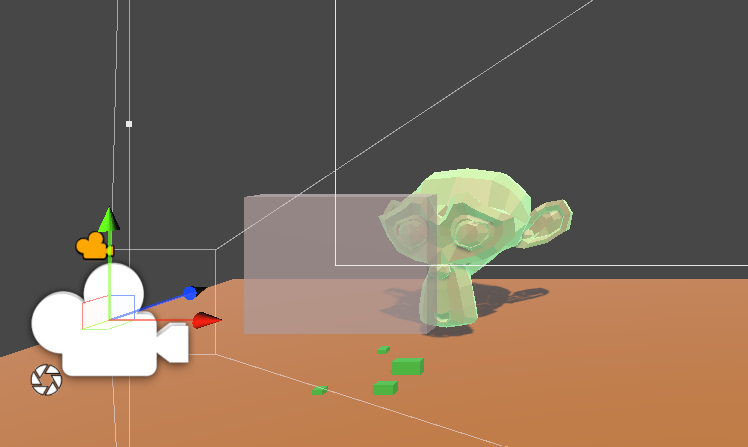
\includegraphics{Scene_1.png}}
\advisor{Marcus Hudritsch}
\expert{Some expert}
\degreeprogram{Bachelor of Science in Computer Science}
\setupSignature{
	A. Muster={
\includegraphics[width=.5\linewidth]{sig_muster}},
	C. Example={
\includegraphics[width=.5\linewidth]{sig_example}}
}


%----------------  BFH tile page   -----------------------------------------
\maketitle
%------------ ABSTRACT        ----------------
\addchap{Abstract}

In meiner Projektarbeit m\"ochte ich einen tieferen Einblick erhalten wie Augmented Reality an einem eigentlich einfachen Anwendungsfall umgesetzt werden kann.\\ Der Betrachter welcher vor einem Bildschirm steht, wird von einer Intel Realsense Kamera D435 erfasst und dessen Position relativ zur Kamera wird ermittelt. In einer virutellen Szene, welche mittels der Gameengine Unity dargestellt wird, wird die Position von der getrackten Person auf eine virutelle Kamera gemappt. Der Blick der virtuellen Kamera entspricht dem Blick des Betrachters. In dieser Szene wird nun ein virtuelles Fenster dargestellt. Dieses Fenster wird perspektivisch in 2D dargestellt und erscheint als verzerrtes Rechteck - je nach Betrachtungswinkel. Nun soll dieses Polygon entzerrt und dann auf dem Bildschirm vor dem Betrachter dargestellt werden. \\ Dem Betrachter erscheint so auf dem Bildschirm ein virtuelles Fenster, deren sichtbare Objekte sich mit der Position des Betrachters perspektivisch verschieben. Der Betrachter soll sich visuell vor einem Fenster in eine virtuelle Welt empfinden.



%------------ TABLEOFCONTENTS ----------------
\tableofcontents

%------------ START MAIN PART ------------
\mainmatter

\chapter{First Thesis Chapter}
\section{Einführung}

Bilder faszinieren mich schon sehr lange. Anfangs waren es Gemälde, Zeichnungen, Skizzen, analoge Fotografien, später dann digitale Bilder und bewegte Bilder. \\ 
Ich bin nun in der Vertiefung Computer Perception and Virtual Reality an der BFH Bern. Im Gespräch mit dem Dozenten Marcus Hudritsch kamen wir auf die Thematik von Raum- und Farbempfinden im Zusammenhang mit Augmented Reality. Es ging darum ein Projektthema zu finden in dieser Vertiefung der Informatikausbildung. \\
Marcus Hudritsch hat mir dann von dieser Umsetzung erzählt: Ein Bildschirm welcher ein künstliches Fenster in eine virtuelle Welt suggeriert.
Ich stelle mir vor, der Betrachter steht etwas verwirrt vor diesem Screen und begreift erst allmählich. Zuerst begreift er, dass sich diese Szene auf dem Screen bewegt, dann nach einigem hin- und hergehen, dass sich die Szene mit ihm im Gleichschritt bewegt und dann nach genauem Beobachten, wie sich die virtuellen Objekte verändern. Dass die perspektivische Darstellung stimmt und es ist, als schaue er durch ein Fenster in eine künstliche Welt von Objekten. \\ Details werde ich in dieser Arbeit später aufzeigen. Wichtig ist mir hier deutlich zu machen, dass es in dieser Umsetzung auch darum geht, den Betrachter von der Realität in die Virtualität hinein zu begeleiten und etwas ins Grübeln zu bringen. \\ Dies wird nur gelingen wenn die Illusion von einem Fenster unserem gewohnten Empfinden gerecht wird und es sich als Realtime Simulation anfühlt.

\section{Komponenten}

\subsection{Physische Komponenten}

\subsubsection{Intel RealSense D435}

\begin{figure}[hbt!]
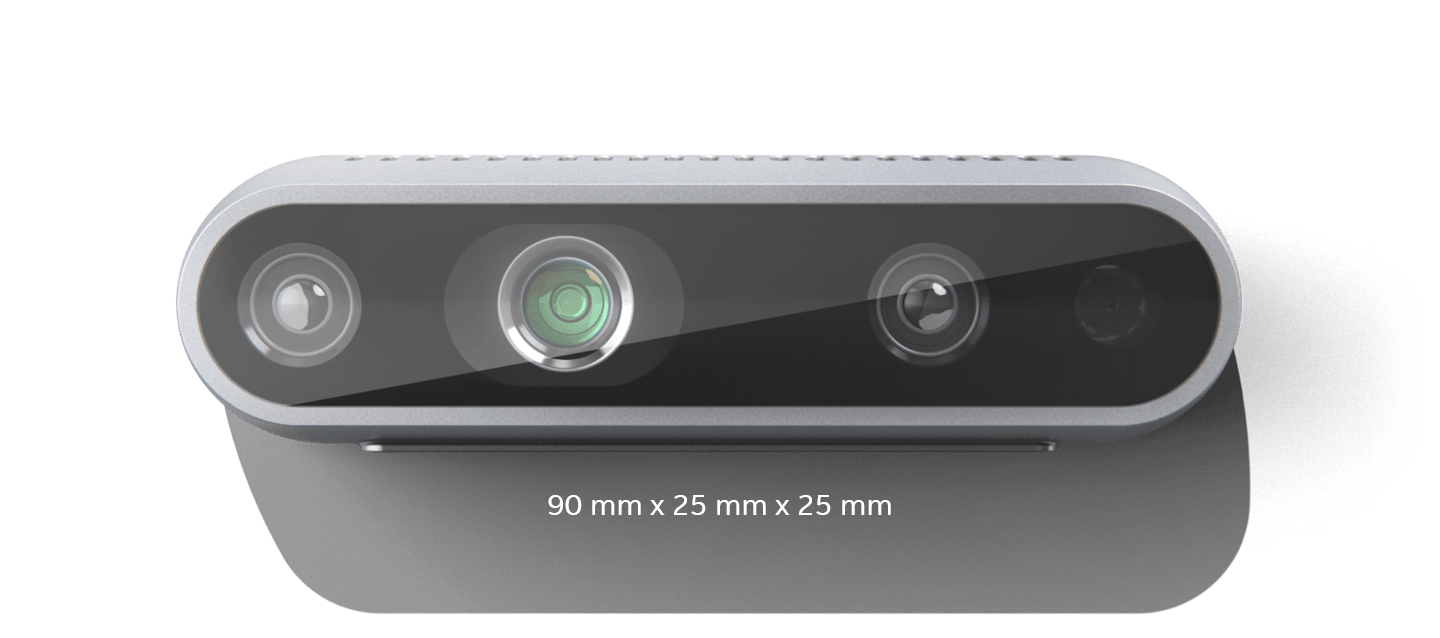
\includegraphics[width=0.6\linewidth]{435d}
\caption{Intel RealSense D435, Frontside}
\end{figure}

Die Kamera D435 von Intel hat ein breites Sichtfeld, einen globalen Shutter und einen Tiefensensor, der sich f\"ur Anwendungen mit schnellen Bewegungen eignet. Gerade durch ihr breites Sichtfeld eignet sich die Kamera fÃŒr Anwendungen in der Robotik, Virtual und Augmented Reality, bei Szenen wo es darum geht m\"oglichst viel zu sehen. Sie hat eine Reichweite bis zu 10 Meter. Das Intel RealSenseSDK bietet plattformunabh\"angig Unterst\"uzung bei der Umsetzung.
			
\begin{figure}[hbt!]
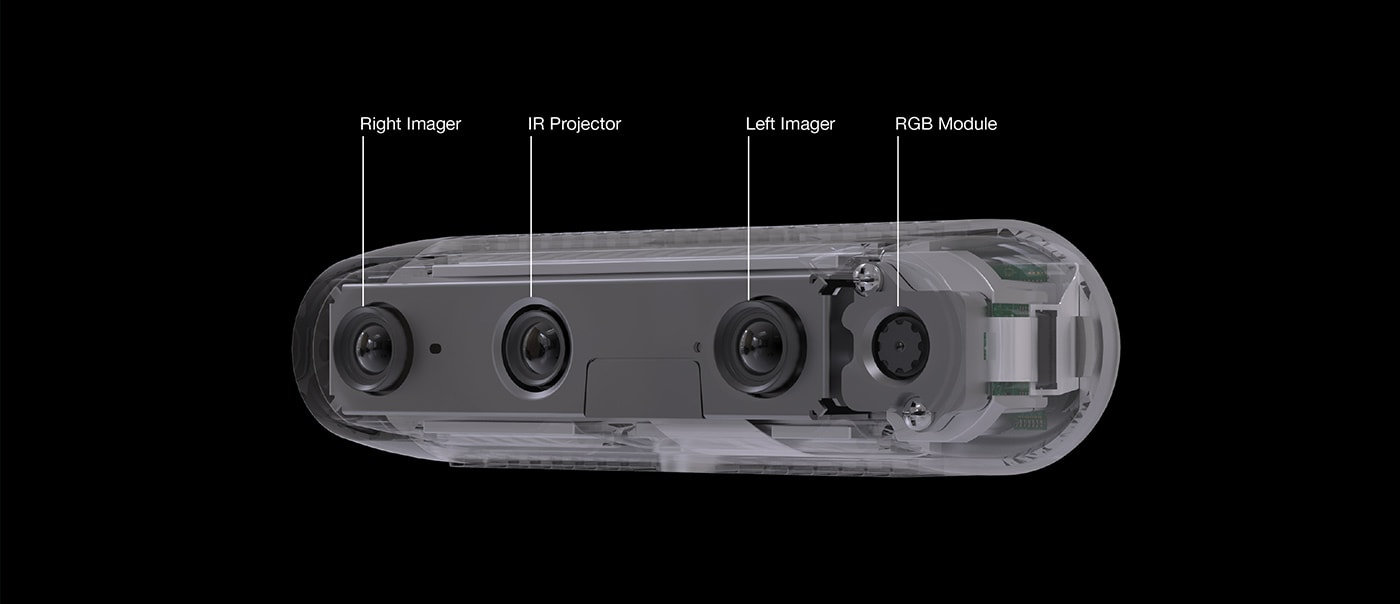
\includegraphics[width=0.6\linewidth]{435d_back}
\caption{Intel RealSense D435, Backside}
\end{figure}
			
Die Global-Shutter-Sensoren haben eine hohe Lichtempfindlichkeit bei schlechten Lichtverh\"altnissen und erm\"oglichen die Steuerung von Robotern auch in dunklen R\"aumen.
\cite{Intel}

\subsection{Software Komponenten}

\subsubsection{Intel RealSense Viewer}

Der Intel RealSense Viewer hat zwei Frames die er anzeigen kann, den RGB Frame und den Depth Frame. Die Abbildung zeigt einen Screenshot vom Depth Frame.

\begin{figure}[hbt!]
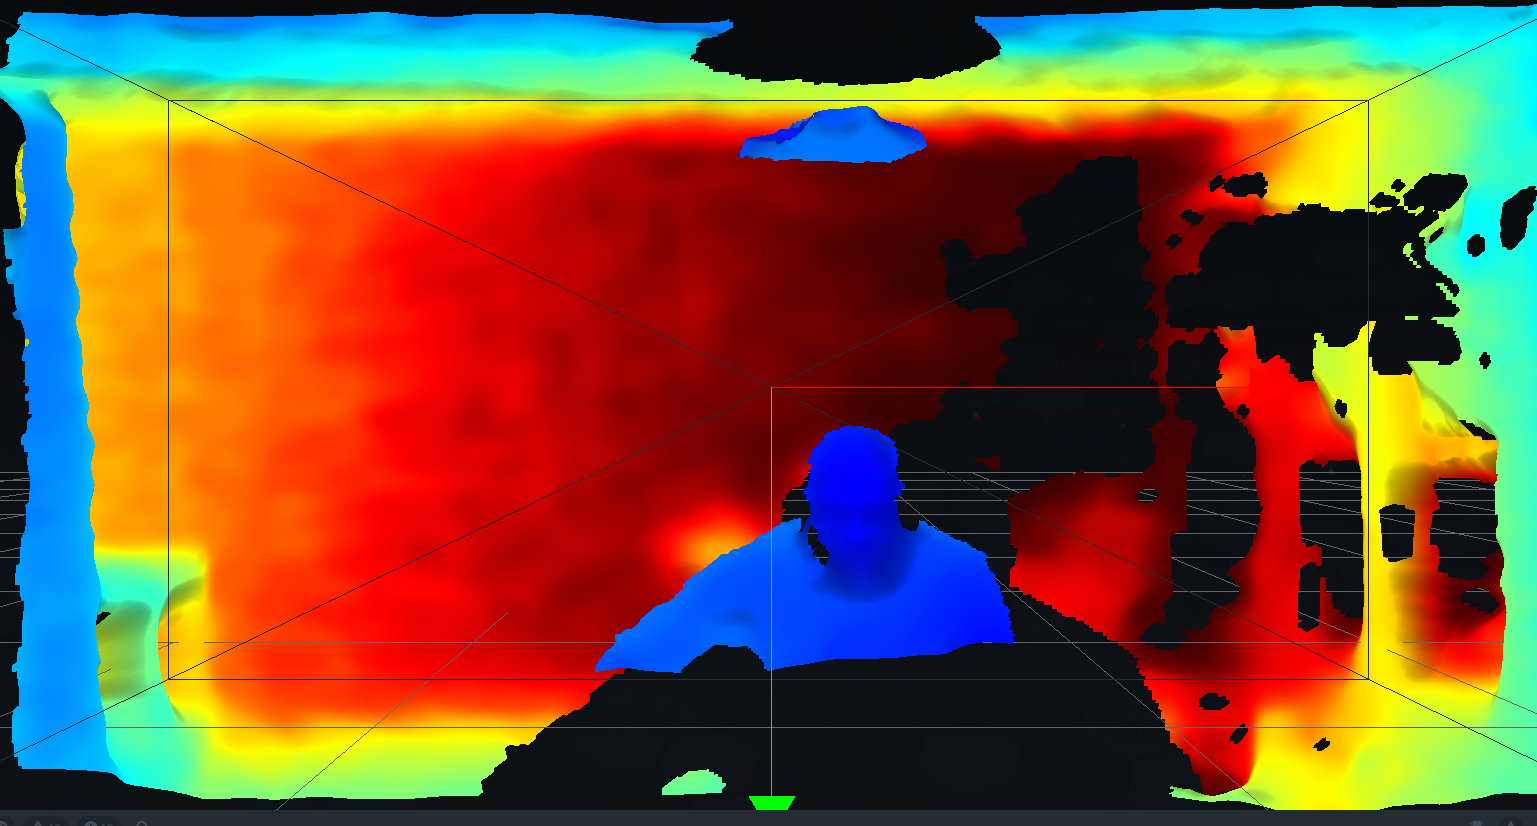
\includegraphics[width=0.6\linewidth]{depth_sensor}
\caption{Intel RealSense Viewer, Depth Frame}
\end{figure}
		
Die blauen Farbpixel zeigen einen nahen Bildpunkt, die roten Farbpixel einen entfernten Bildpunkt. F\"ur mein Projekt eignent sich dieser Viewer einzig dazu die verschiedenen Kameraeinstellungen auszuprobieren.
			
\subsubsection{Intel RealSenseSDK 2.0}

Intel hatte vor einigen Jahren eine f\"uhrende Rolle in Anwendungen im Bereich Augmented Reality. Mit dem Intel RealSenseSDK 2016, dem Vorgänger vom RealSenseSDK 2.0 gab es ein ToolKit welches Facetracking implementiert hatte. Die rechte und die linke Hand konnte beispielsweise seperat fürs Tracking angesteuert werden und sogar einzelne Finger einer Hand konnten getrackt werden. \\Ich habe noch versucht dieses "\"altere SDK zu installieren und dann mit einer \"alteren Unity Version zu verwenden. Leider ohne Erfolg. Intel hatte eine ganze Videoreihe dazu erstellt, welche aber heute vom Netz genommen wurden.\\
Intel schließt seine Abteilung rund um die RealSense-Kameras, die viele Jahre interessante, aber vom Markt kaum umgesetzte Lösungen hervorgebracht hatte. Sie passt nicht zum neuen Geschäftsmodell, welches rund um die Kernthemen von Intel aufgebaut und von dem neuen Foundry-Geschäft unterstützt wird.
\cite{ComputerBase}- \\ Das neue SDK 2.0 taugt dagegen nur noch wenig und eignet sich nicht f\"ur mein Projekt. Das Toolkit implementiert kein Facedetection für Unity Anwendungen.			

\subsubsection{Unity}

Unity ist eine Game Engine die von einer Open Source Community betreut und weiterentwickelt wird. Unity bietet f\"ur dieses Projekt ein anwendungsfreundliches Toll mit welchem die Transformationen der Objekte gemacht werden k\"onnen. \\ Dies w\"are auch mit OpenGL m\"oglich. OpenGL ist die eigentliche Mutter aller Grafik Softwares. \\In Unity ist es dann auch m\"oglich komplexe Objekte mit unterschiedlichen Oberfl\"achen und Texturen mit der gew\"unschten Lichtsituation darzustellen. 
\cite{Unity}
			
			
\subsubsection{Nuitrack}

Nuitrack stellt in ihrem SDK viele Anwendungen zur Verf\"ugung, diese sind aber auf 3 Minuten Spieldauer limitiert. Wahrscheinlich haben sie von Intel gelernt und haben ein Pricing welches f\"ur volle Anwendungen \$99.99 pro Jahr kostet. In der nächsten Abbildung sind alle implementierten Features dargestellt.

\begin{figure}[hbt!]
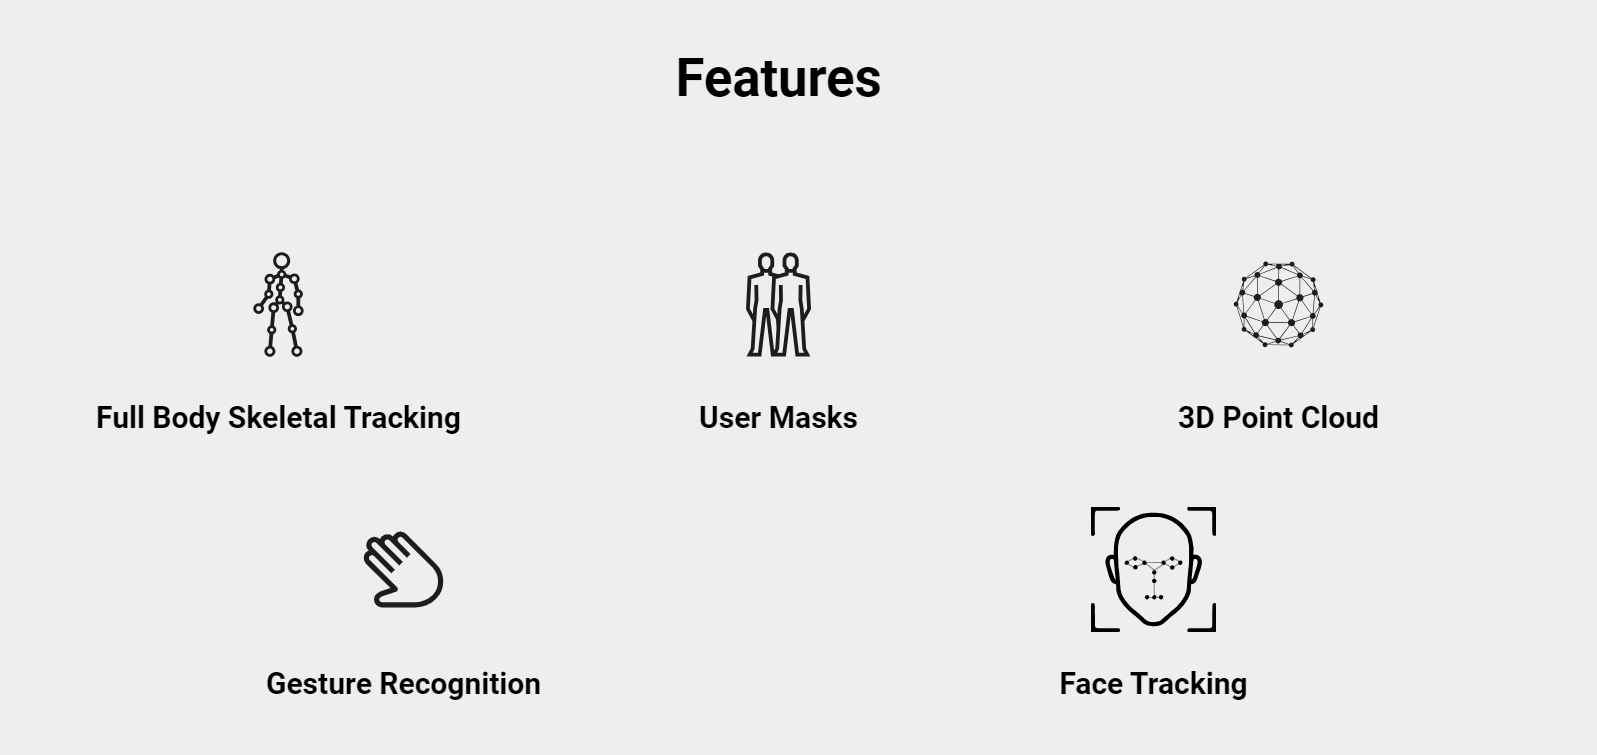
\includegraphics[width=0.6\linewidth]{nuitrack_features}
\caption{Nutitrack SDK, Features}
\end{figure}

Dieses SDK ist enorm m\"achtig und hat alles zu bieten, was ich für mein Projekt brauche. Wichtig für mein Projekt ist das Facetracking und das Full Body Skeletal Tracking. Die Nutirack SDK hat eine gute Anbindung zu Unity und ist gut domumentiert.
\cite{NuitrackSDK} 

\subsection{OpenCV}

OpenCV ist eine Open Source Computer Vision Grafik Library. In meinem Projekt benötige ich diese Library um ein bliebiges Polygon mit Seiten zu entzerren und als Rechteck darzustellen. Es gibt einen Wrapper für diese Library, welcher sich in Unity einbinden lässt. 
Dieser ist kostenpflichtig. Herr Hudritsch konnte mir eine Free Version geben, dies im Rahmen der Ausbildung.
Informationen zu OpenCV finden sich unter: https://opencv.org/ und für das Unity Plugin unter: https://enoxsoftware.com/opencvforunity/.
			
\subsection{Homographie}

\vspace{0.5in}

\begin{figure}[hbt!]
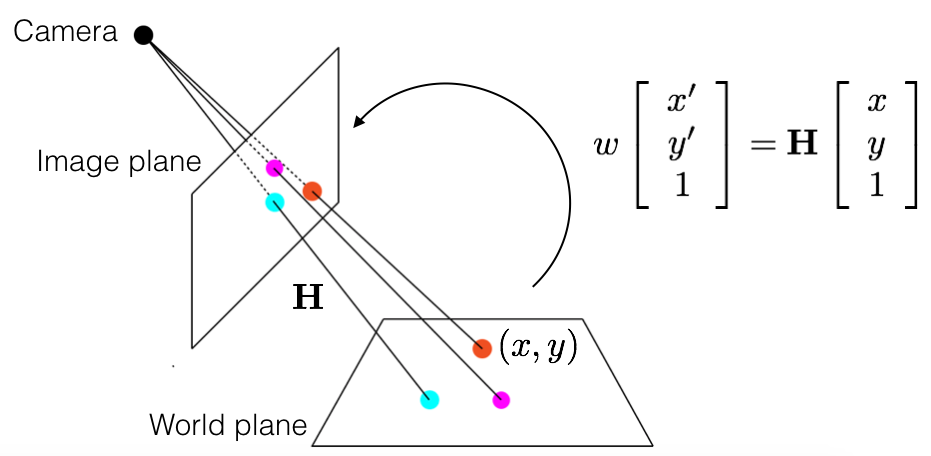
\includegraphics[width=0.6\linewidth]{homography}
\caption{Homographie, Visualisation}
\end{figure}
		
Die Homographie Matrix H beschreibt wie die Originalpunkte x,y zu liegen kommen in der Bildebene. Die Homographie Matrix ben\"otigt jeweils 4 Punkte in der Quellebene und die entsprechenden Punkte in der Zielebene. \\ 
		
			
\begin{figure}[hbt!]
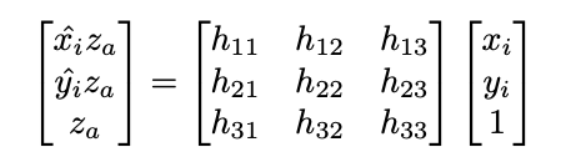
\includegraphics[width=0.6\linewidth]{homography_abbildung}
\caption{Homographie, Abbildungsgleichung}
\end{figure}
		
Diese 8 Punkte werden als Vektoren in einer Matrix A dargestellt. Die Matrixmultiplikation von A mit der Homographie Matrix die wir suchen, wird in einem Gleichungssystem von 8 Gleichungen und 8 Unbekannten gelöst.
			
			
\begin{figure}[hbt!]
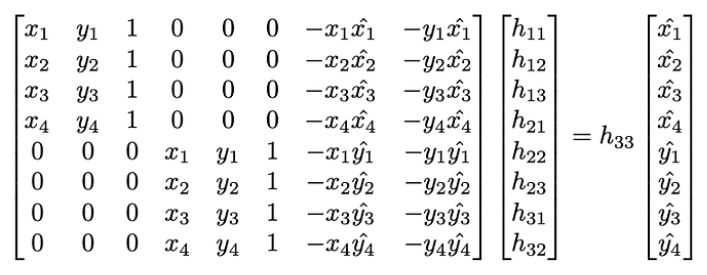
\includegraphics[width=0.6\linewidth]{homography_gleichungssystem}
\caption{Homographie, Gleichungssystem}
\end{figure}
		
Der Streckungsfaktor h33 zeigt, dass die Homographie Matrix noch skaliert werden kann. Im Default Fall wird h33 eins gesetzt.
\cite{OntarioTech}
\cite{HomographyEstimation}
			
\subsection{Kameramodell}

\vspace{0.5in}

Um auf die Eckpunkte vom Screen zu kommen, sollte es reichen, wenn wir die Position der Kamera, deren Rotationswinkel, sowie den Winkel vom Field of View und den Viewport der Kamera kennen. Weiter kennen wir die World Positions von den Eckpunkten vom Screen. Da der Screen statisch ist und sich nicht bewegt, können wir dieses Model ausser acht lassen. Was bleibt ist: der Viewport (1), die Projektion (2) (Kamera intrinsisch) und das Kamera-Modell (3) (Kamera extrinsisch oder View).
Unsere Abbildungsmatrix ist also:
Matrix m = (1) * (2) * (3)
Und mittels Anwendung auf die Eckpunkte vom Screen:
P1' = P1 * m

\section{Results}
What did you find? – a section which describes the data that was collected and the results of any statistical tests that were performed.  It may also be prefaced by a description of the analysis procedure that was used. If there were multiple experiments, then each experiment may require a separate Results section.


\chapter{Second Thesis Chapter}
\section{Ergebnisse}

\subsection{Einbinden von Nuitrack}
Nuitrack kann unter folgendem Link für alle Platformen runtergeladen werden: \href{https://github.com/3DiVi/nuitrack-sdk/blob/master/doc/Install.md}{\textbf{Nuitrack}}. \\ Die Software ist Platform unabhängig verfügbar und wird im gewünschten Folder auf der Festplatte installiert.

\subsubsection{Import Nuitrack Wrapper in Unity}
Unter folgendem Git Repo kann das Nuitrack Plugin runtergeladen werden: \href{https://github.com/3DiVi/nuitrack-sdk/blob/master/Unity3D/NuitrackSDK.unitypackage}{\textbf{Nuitrack Unity Plugin}}. Da dieses Plugin für verschiede Sensoren, also Kameras konfiguriert wurde, muss dann noch der Sensor spezifiziert werden. In meinem Projekt ist dies das Plugin für die IntelRealsense D435 Kamera.


\subsubsection{Skeleton Tracking mit NuitrackSDK}
Das Tutorial von Nuitrack ist meine Ausgangslage um eine Person zu tracken. Der Link führt zu diesem Tutorial: \href{https://github.com/3DiVi/nuitrack-sdk/blob/master/doc/Unity_Face_Tracking.md}{\textbf{Nuitrack Facetracking}}. \\ Das Tutorial ist gut beschrieben und lässt sich genau so umsetzen wie beschrieben.

\subsection{Virtuelle Szene in Unity}

\begin{figure}[H]
	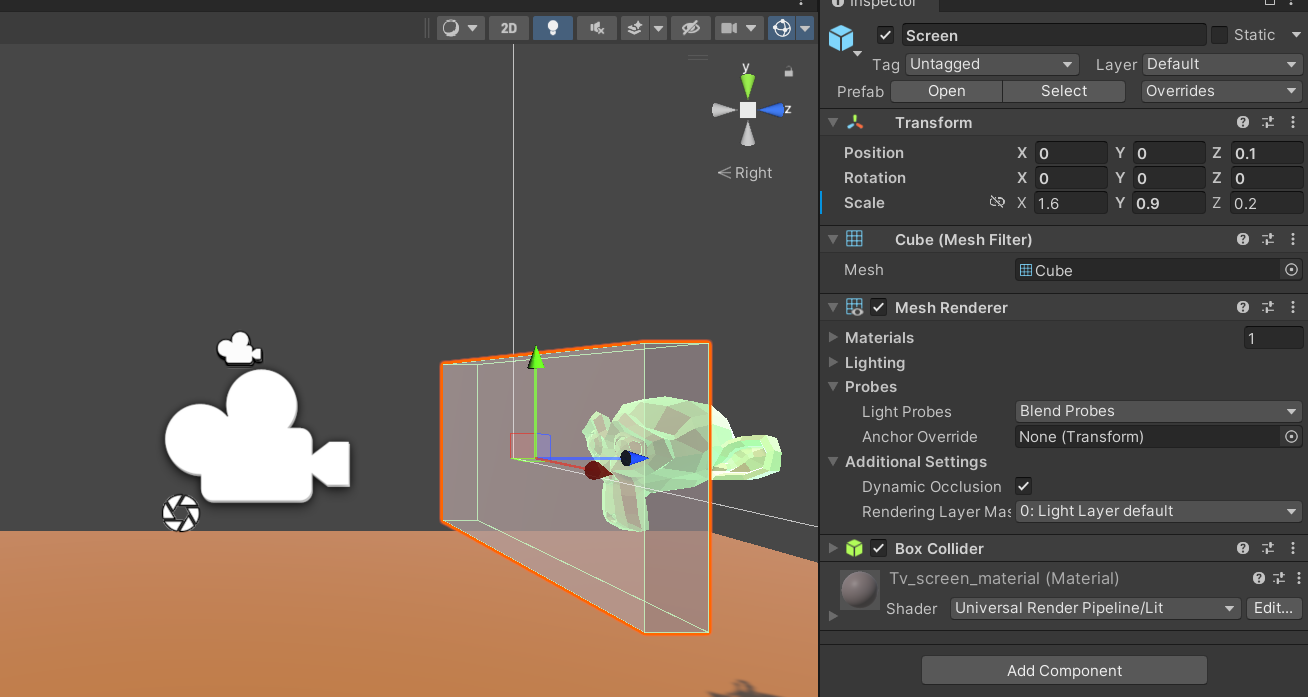
\includegraphics[width=1.0\linewidth]{Screen}
	\caption{Unity, Szene}
	\label{fig:Screen}
\end{figure}

In Unity baue ich die Szene so auf, dass die Render-Kamera in positiver z-Achse ausgerichtet ist. Anfangsposition der Render-Kamera ist (0, 0.2, -1.5). Den Screen welcher dann entzerrt werden soll, setze ich auf den Nullpunkt. Die Mitte vom Screen hat die Position (0, 0, 0).
Die Eckpunkte vom Screen haben die folgenden Positionen: 
P0(-0.8, -0.45)
P1( 0.8, -0.45)
P2( 0.8,  0.45)
P3(-0.8,  0.45)
Der Screen hat die Grösse 1600 x 900 mm. Dieser wird als schmaler Kubus dargestellt und transparent leicht grau eingefärbt, damit ich dann erkennen kann ob mein Rendern und Entzerren richtig funktioniert.
Die Main-Kamera setze ich als Referenz auf die Position der Render-Kamera. Dies damit ich eine Ansicht in der Szene bekomme. Die Main-Kamera zeigt dann die Szene und in der Game Ansicht zeigt die Render-Kamera den Output vom entzerrten Screen.  
Gut möglich, dass man dies auch mit weniger Kameras darstellen kann. \\ Figure~\ref{fig:Screen} zeigt den Aufbau der Szene mit dem grau eingefärbtem Screen und dessen Werte im Inspektor Fenster rechts daneben.

\subsection{Render Kamera zeigt Position vom Betrachter}
Die Render-Kamera wird als Referenz auf den obersten Knochen vom Skelett gemappt. Dieser oberste Knochen entspricht dem Kopf, genauer der Stirn.
Damit wird dann auch die Main-Kamera, welche die Render-Kamera referenziert auf den Kopf gemappt.

\subsection{Render Kamera zeigt RenderTexture}
Die Render-Kamera wird nun stets auf den Mittelpunkt vom Screen gerichtet. Der Output der Render-Kamera erzeugt dann eine RenderTexture der Grösse 750 x 750 Pixel. Je grösser die Anzahl Pixel, desto besser wird dann die Qualität vom Endbild.

\begin{figure}[H]
	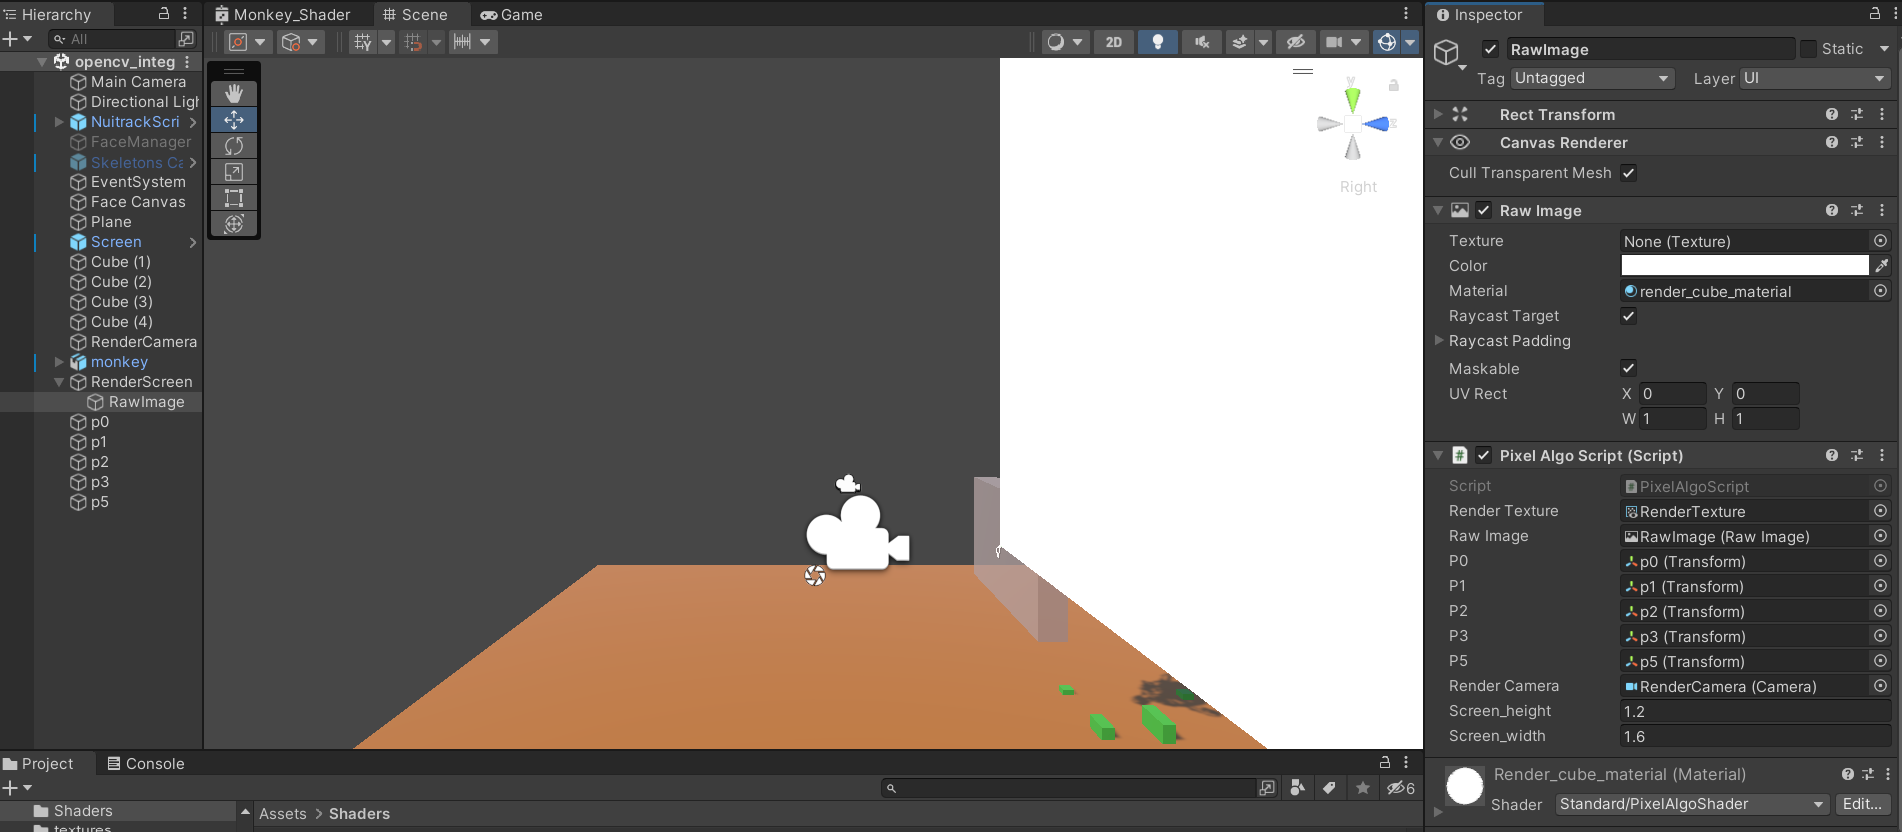
\includegraphics[width=1.0\linewidth]{RawImage}
	\caption{Unity, RawImage}
	\label{fig:Rawimage}
\end{figure}

Figure~\ref{fig:RawImage} zeigt das Output Bild, welches auf der weissen Ebene dargestellt wird. Diese entspricht nun dem Output Bild für den Screen und zeigt ein Format 16 : 9.


\subsection{Matrix Shader}
Im Netz habe ich einen Rotations Shader gefunden und versucht diesen so anzupassen, dass die Entzerrung gelingt. Leider ohne Erfolg. Das Probelm bei diesem Shader: Zwar funktioniert das Scaling und das Shearing, leider nicht aber die Translation.
Ich habe dann versucht eine Translation hinzuzufügen, was auch funktioniert hat.  

\begin{figure}[H]
	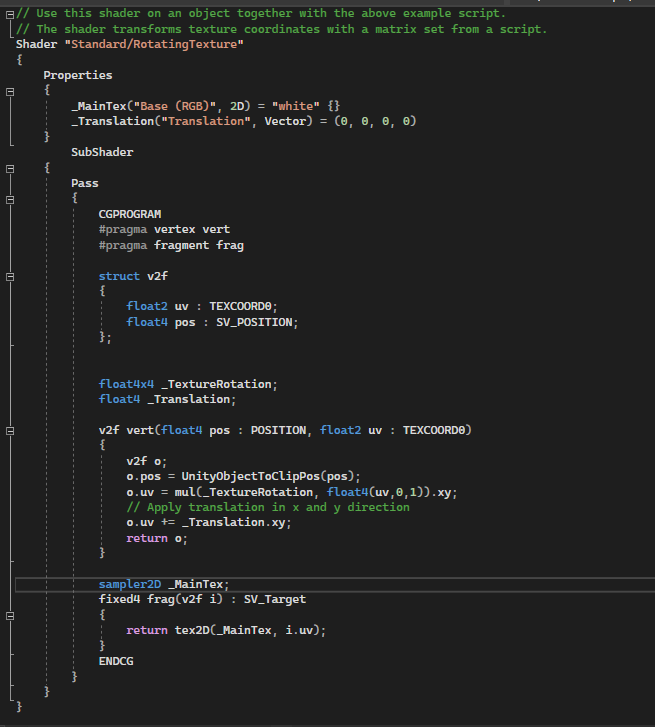
\includegraphics[width=0.8\linewidth]{Rotationsshader}
	\caption{Unity, MatrixShader}
	\label{fig:MatrixShader}
\end{figure}


Figure~\ref{fig:MatrixShader} zeigt den umgebauten Matrix-Shader mit einer Möglichkeit die x und y Koordinaten der Pixel zu verändern.
Leider weiss ich aber nicht, wie ich mit dieser Rotationsmatrix das Polygon selektieren soll und dann entzerrt darstellen.
Als Einstieg in die Unity Shader hat es trotzdem etwas geholfen, mehr aber auch nicht.

\subsection{Pixel Shader}
Damit ich diese Entzerrung vom Polygon machen kann, benötige ich einen Pixel-Shader. Oder einen Shader welcher die Maintexture ändert.
Ich erstelle nun so Schritt für Schritt einen Shader welcher als Parameter die Maintextur als Eingabewert hat. Und diese Maintexture dann im Shader jeweils angepasst wird. \\  Im Script wird in der Update Funktion für jedes Pixel der Farbwert gesetzt und am Ende die Textur dem Shader übergeben.


\begin{figure}[H]
	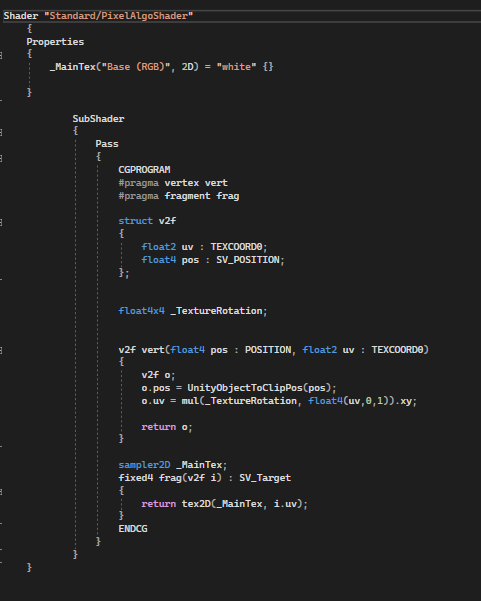
\includegraphics[width=0.8\linewidth]{PixelAlgoShader}
	\caption{Unity, Pixel-Shader}
	\label{fig:PixelShader}
\end{figure}

Figure~\ref{fig:PixelShader} zeigt den Shader, welcher die Texturen verändert, indem die Pixelwerte der Maintexture verändert werden.

\subsection{Homographie}
Unter dem folgenden Link habe ich ein Git Repo gefunden, welches die Homographie Matrix mit Gauss Elimination durchführt: 
\href{https://github.com/chiragraman/Unity3DProjectionMapping/blob/master/Assets/Scripts/Homography.cs}{\textbf{Homographie Matrix Berechnung}}.
Zuerst habe ich versucht die Entzerrung mit einer Homographie Matrix zu erreichen. Leider hat dies nur geklappt für die Ansicht ohne seitliche Verschiebung, also mit einem x-Wert von Null. Sobald ich etwas abweiche von dieser zentralen Position, zeigt sich ein Shearing im Output Bild, welches sich auch noch anders verhält, je nachdem ich in positiver x-Achse gehe oder in negativer x-Achse. 
Ich habe da länger darüber nachgedacht, meine Homographie Matrix mehrmals geprüft, fand aber nicht heraus was das Problem war. Komisch ja auch, dass es in zentraler Position den richtigen Output gab, bei seitlicher Verschiebung sich dann aber ein Shearing zeigt, welches mit grösserer Abweichung nach links oder rechts dann auch noch grösser wurde.
Somit brauche ich nun einen anderen Ansatz um die Entzerrung zu lösen.

\subsection{OpenCV}
OpenCV hat bereits Methoden, welche diese Entzerrung vornehmen. Das Plugin von OpenCV findet sich unter: \href{https://github.com/EnoxSoftware/OpenCVForUnity/tree/master/Assets/OpenCVForUnity}{\textbf{OpenCV Unity Plugin}}.
Die grösste Schwierigkeit ist bei OpenCV, dass Unity einen anderen Aufbau der Matrizen hat und dass OpenCV keine Textures kennt. 
Die grösste Schwierigkeit war dann zu merken, dass die Pixelwerte der Textures in OpenCV nicht einfach so auf der CPU verfügbar sind. Diese werden auf der GPU gespeichert und mössen dann exklusiv abgefragt werden.
Die Funktionen von OpenCV funktionieren tadellos. Damit die Entzerrung gelingt, gehe ich vom Zielbild aus und berechne die Perspektivische Matrix rückwärts vom Zielbild zum Inputbild, was dann dem Inversen der Perspektivischen Matrix entspricht. 
Nun wird diese Matrix auf jedes Pixel des Zielbildes angewendet und so den Farbwert an der entsprechenden Stelle im Inputbild geholt. 
Da diese Operation mit der Anzahl Pixel steigt, habe ich hier ein Format vom Zielbild 800 x 450 Pixel gewählt.

\begin{figure}[H]
	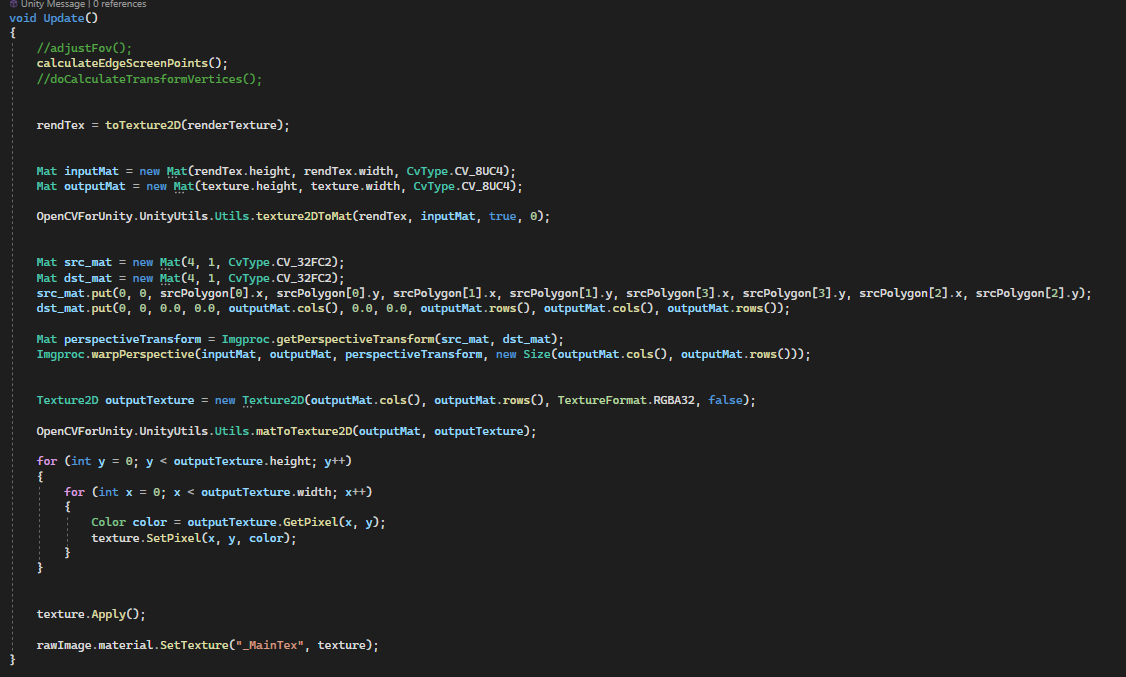
\includegraphics[width=1.0\linewidth]{OpenCV}
	\caption{Unity, OpenCV}
	\label{fig:OpenCV}
\end{figure}

In Figure~\ref{fig:OpenCV} zeigt sich diese Problematik. Die Textures werden in OpenCV Mat, also Matrizen umgewandelt. Die wichtigen Methoden von OpenCV sind dann: \\  
Mat perspectiveTransform = Imgproc.getPerspectiveTransform(srcMat, dstMat); \\
In getPerspectiveTransform wird die Homographie-Matrix anhand der vier Quellpunkte und der vier Zielpunkte berechnet. Die andere wichtige Methode von OpenCV: \\ 
 Imgproc.warpPerspective(inputMat, outputMat, perspectiveTransform, new Size(outputMat.cols(), outputMat.rows())); \\ In dieser warpPerspective Methode passiert die Entzerrung. In outputMat ist dann die gewünschte, entzerrte Textur, aber noch nicht als Textur. Deshalb wird dann diese OpenCV Mat in eine Textur umgewandelt. \\ Damit überhaupt etwas angezeigt wird braucht es nun noch diese explizite Abfrage der Pixelwerte, welches im Code in der For Schleife passiert.  \\ Am Ende wird die neu generierte Textur dem Pixel-Shader übergeben. Dies passiert mit der letzten Zeile: \\
 rawImage.material.SetTexture(" MainTex", texture);

\subsection{Kameramodell}
Ich habe versucht mittels Kameramodell die Transformationsmatrix für die Eckpunkte vom Screen zu berechnen. Dazu braucht man den Viewport, die intrinsiche (Projektionsmatrix) und die extrinsische Kameramatrix (Viewmatrix). Da sich der Screen nicht verschiebt, braucht es die Modellmatrix nicht.

\begin{figure}[H]
	\includegraphics[width=1.0\linewidth]{KameraMatrix}
	\caption{Unity, Berechnung Kameramatrix}
	\label{fig:Berechnung Kameramatrix}
\end{figure}

\begin{figure}[H]
	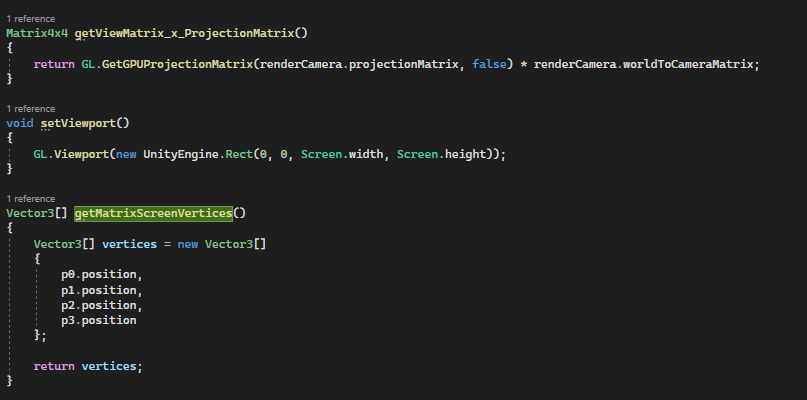
\includegraphics[width=1.0\linewidth]{Kameramatrix2}
	\caption{Unity, Methoden Kameramatrix}
	\label{fig:Kameramatrix Methoden}
\end{figure}

In Figure~\ref{fig:Berechnung Kameramatrix} versuche ich die Kamera-Matrix zu berechnen, wie bereits im Kapitel Kameramodell beschrieben.

\subsection{Projektion der Eckpunkte auf der Zielebene}
Mein Ansatz den ich umgesetzt habe funktioniert wie folgt: 
Unity hat eine Funktion welche mir die Eckpunkte von der Clipping Ebene entsprechend dem z Wert herausscheibt. Ich wähle diese Ebene durch den Nullpunkt, auf welchen sich die Render-Kamera immer richtet. 
Nun projeziere ich die Eckpunkte vom Screen in der Verlängerung von der Render-Kamera durch die Eckpunkte. Die Schnittpunkte mit der Ebene müssen nun nur noch relativ zu den Ecken der Clipping Ebene berechnet werden. 







\section{Discussion}
What is the significance of your results? – the final major section of text in the paper.  The Discussion commonly features a summary of the results that were obtained in the study, describes how those results address the topic under investigation and/or the issues that the research was designed to address, and may expand upon the implications of those findings.  Limitations and directions for future research are also commonly addressed.

\section{Fazit}


\section{Ausblick}
In einer nächsten erweiterten Umsetzung, könnte ich mir vorstellen, dass der Eindruck von einem virtuellen Fenster noch gesteigert werden kann. \\ Dies indem die virtuelle Szene mit zwei Kameras, eine Kamera fürs linke Auge und eine Kamera fürs rechte Auge die virtuelle Szene filmt. Nun müssten die beiden Bilder in einer Updatemethode von Unity abwechselnd eingespielt werden. Da die update Frequenz deutlich grösser ist, als das menschliche Auge feststellen kann, könnte ich mir vorstellen so einen 3D Effekt der Szene für den Betrachter erzeugen zu können. Hier gibt es aber dann noch ein Problem: Die rechte und die linke Kamera erhalten nicht ganz die gleichen Eckpunkte für den gerenderten Screen. Möglicherweise helfen da Durschnittswerte beider Kameras. Es wäre also interessant zu sehen ob dieser Ansatz wirklich funktioniert.


%------------ Authorship declaration translated to main language ------------
\declarationOfAuthorship

%----------- Bibliography ----------------
\clearpage
\bibliographystyle{unsrt}
\bibliography{project}      % the project.bib file gets loaded

%------------ List of Figures ------------
\listoffigures
 
%------------ List of Tables -------------
\listoftables
 
%------------ List of Listings -----------
\lstlistoflistings 
 
%------------ Glossary -------------------
\printglossary

%------------ Index ----------------------
\clearpage
\printindex
%------------ Appendix ----------------	
\appendix
\chapter{First Appendix Chapter}

\end{document}
